\documentclass[11pt,a4paper]{article}

\usepackage[margin=0.85in]{geometry}
\usepackage{graphicx}
\usepackage{booktabs}
\usepackage{amsmath}
\usepackage{hyperref}
\usepackage{float}
\usepackage{caption}
\usepackage[T1]{fontenc}
\usepackage{lmodern}
\usepackage{microtype}
\usepackage{enumitem}

\captionsetup{font=small,skip=2pt}
\setlength{\parskip}{2pt plus 0.5pt}
\setlength{\parindent}{1em}
\setlist{nosep,leftmargin=1.2em}
\setlength{\textfloatsep}{4pt plus 1pt minus 1pt}
\setlength{\intextsep}{4pt plus 1pt minus 1pt}

\graphicspath{{../data/analysis/}}

\title{Plurality Collapse: Structural Compression, Categorical Limits, and Surface Confounds\\[0.3em]\large Milestone 3 Report}
\author{Xan Carey (yac2014), Kevin Huang (qh2257@nyu.edu), Quinn Pu (quinn.t.s@nyu.edu)}
\date{May 2026}

\begin{document}
\maketitle
\vspace{-1em}

%% ============================================================================
\section{Methodology}
%% ============================================================================

Milestone 2 reported a 35--41\% gap in the geometric dimensionality of human vs LLM rationales embedded in Kaleido-XL~\cite{sorensen2024kaleido} and called it ``plurality collapse''. Throughout, we measure dimensionality as comp90, the number of principal components needed to capture 90\% of a corpus's variance. Milestone 3 runs five probes designed to falsify the original claim, expands the human corpus, and decomposes what survives.

The five probes are a permutation null on shuffled source labels (tests whether the gap is chance), iterative null-space projection~\cite{ravfogel2020inlp} at 20 iterations (tests whether one low-rank axis carries the gap), a per-component analysis on the pooled embeddings (tests how variance is distributed across PCs), Ridge regression of the embedding on TF-IDF + log length followed by subtraction of the prediction (tests how much is linearly predictable from text), and the Moral Foundations Dictionary~\cite{graham2009moral} as a Kaleido-independent diversity measure. We also rewrite 300 human rationales as formal prose and 300 LLM rationales as casual Reddit comments with Qwen 2.5 3B Instruct~\cite{qwen2025}, giving a 4-cell gap matrix that isolates register from content.

The corpus is extended with the ArcticShift Reddit archive~\cite{arcticshift}. We pull 68,391 top-level verdict-bearing human comments across 1,991 dilemmas (median 34 per dilemma) and embed via the same Kaleido pipeline. This gives multiple human rationales per dilemma, so we can compute within-dilemma diversity rather than only cross-dilemma diversity available in the Sachdeva dataset~\cite{sachdeva2025dilemmas}. We stratify by consensus, verdict, length, author, and time, and residualize on TF-IDF + length, character n-grams + function words, author-mean, and model-mean. We compare diversity at three increasingly fine categorical levels (MFD foundations, the 60-cluster Kaleido value taxonomy from milestone 2, and within a single Kaleido cluster). The within-cluster residual is decomposed by three further probes. We extract 22 lexical and pragmatic features per comment. We fit a principal component analysis on 48,297 (human, LLM) difference vectors with a random-pairing baseline. We ask Qwen 2.5 3B Instruct for a one-sentence framing difference on 205 same-cluster pairs.

%% ============================================================================
\section{Results}
%% ============================================================================

\subsection{Corpus Probes}

The dimensionality gap survives the structural tests. The permutation null gives $z{=}77.6$. 87\% of 500 pooled PCs have higher human than LLM variance by a factor of $1.5\times$ or more, and not a single PC shows the reverse. Twenty INLP iterations drive linear source-classification from 0.998 to 0.543 but the comp90 gap grows from 121 to 147 components. No single low-rank axis carries the gap.

But three independent tests show the corpus gap is dominated by register and surface text, not by moral content. Ridge regression on TF-IDF + log length closes the gap from 121 to 11 components, a 91\% reduction, while removing only 12\% of human and 20\% of LLM variance. The MFD-based diversity gradient reverses sign relative to the Kaleido-decoder gradient from milestone 2 ($r{=}+0.897 \to r{=}-0.559$) and survives length stratification. Register-matched paraphrase closes the gap from $+19$ to $-1$. Roughly half of paraphrases drift to a different Kaleido value cluster, so the test conflates register matching with paraphrase content drift. To rule out a generational explanation, Qwen 2.5 3B Instruct generates 1,000 fresh AITA rationales. Qwen lives at comp90 $=219$, near Sachdeva's all-LLM matched-$n$ value of 216, and its centroid is 0.031 from the Sachdeva LLMs vs 0.070 from humans. A 2024 model sits inside the older LLM cluster.

\subsection{Per-Dilemma Diversity}

Holding the dilemma fixed, the mean pairwise cosine within human comments is $0.297 \pm 0.027$ and within LLM rationales is $0.147 \pm 0.020$. Humans are more pairwise-diverse than LLMs in $100\%$ of 1,991 dilemmas, with mean ratio $2.02\times$. The result holds uniformly across consensus level ($1.91$--$2.03\times$), verdict ($1.88$--$2.05\times$), and comment-length quartile ($1.92$--$2.08\times$). The fraction of dilemmas in which humans beat LLMs is exactly $1.000$ in every stratum.

Every control we ran keeps the ratio above $1.5\times$. Ridge regression on TF-IDF + length gives $2.13\times$. Higher-order surface controls (character n-grams + function words + sentence statistics) give $2.02\times$. Replacing Kaleido with sentence-transformers~\cite{reimers2019sbert} gives $2.21\times$. Restricting to NTA-only verdicts gives $2.60\times$. Per-LLM ratios range from $2.3\times$ to $7.8\times$. Subtracting each human's mean embedding across their own comments and each model's mean embedding across its own outputs drops the ratio to $1.56\times$. Roughly 23\% of the gap is therefore author or model stylistic identity, and roughly 77\% is genuine variation within a single dilemma. Splitting by comment time finds no early-vs-late convergence.

The diversity is layered. At the MFD foundation level humans and LLMs invoke near-identical numbers of foundations per dilemma (6.99 vs 6.84). At the Kaleido 60-cluster value level humans use $4.93$ distinct clusters per dilemma vs LLMs $3.39$, a $1.46\times$ gap. And when both pick the same Kaleido cluster on the same dilemma, humans are still $1.95\times$ more pairwise-diverse within that cluster ($n{=}4329$ such pairs, humans beat LLMs in $96.5\%$). The diversity lives mostly inside the cluster rather than in which cluster is chosen.

\begin{figure}[H]
\centering
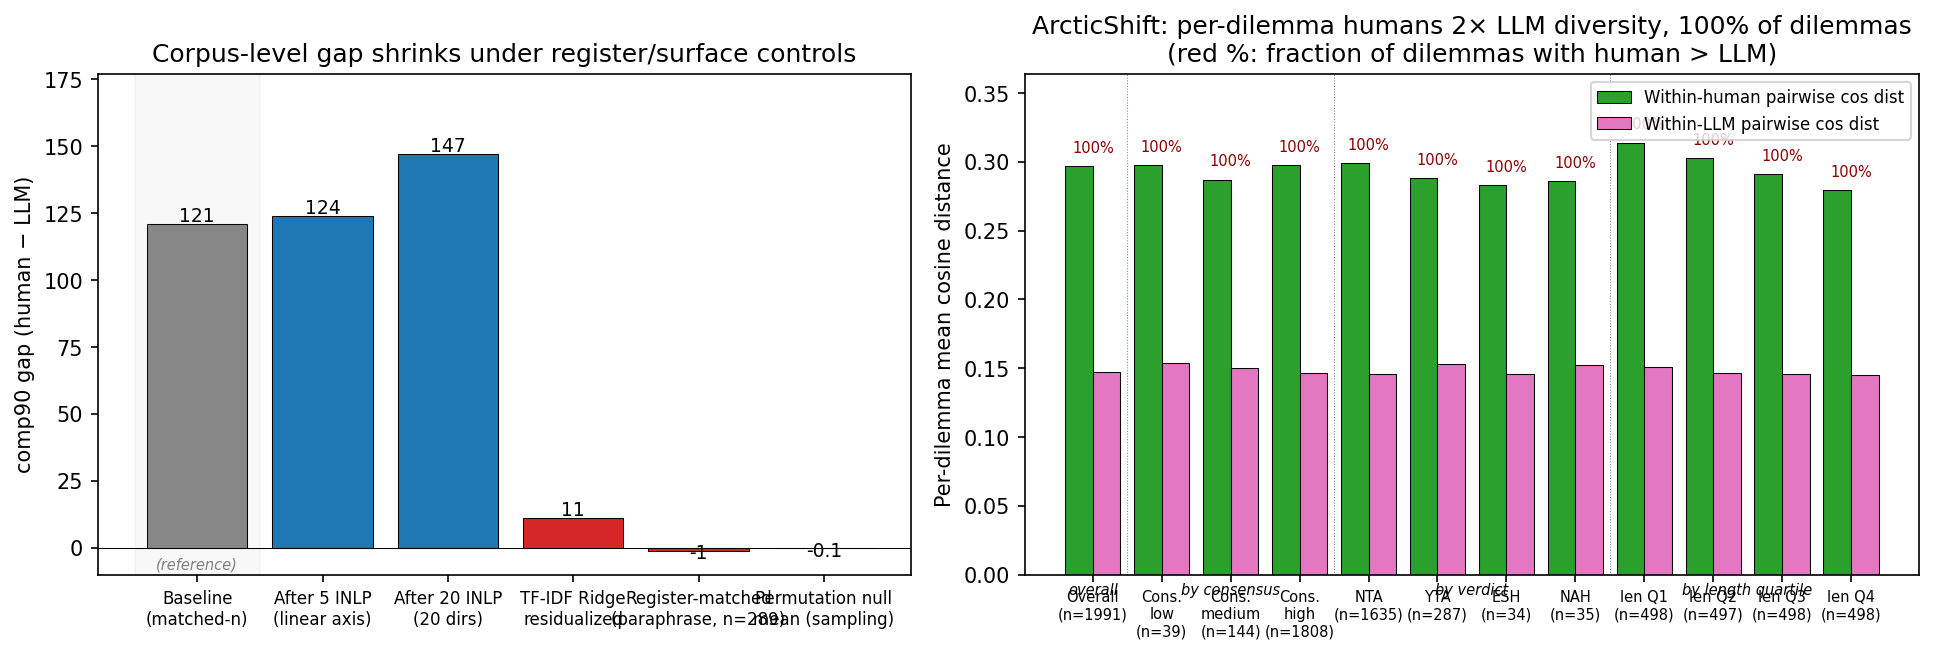
\includegraphics[width=0.92\textwidth]{milestone3_summary.png}
\vspace{-0.5em}
\caption{Left: corpus-level comp90 gap shrinks sharply under register and surface controls but stays far above the permutation null. Right: per-dilemma within-source cosine by consensus, verdict, and length quartile. Frac h$>$l is $1.000$ in every stratum and the ratio is $\sim 2\times$.}
\label{fig:summary}
\end{figure}

\subsection{Framing Decomposition}

The within-cluster $1.95\times$ ratio is decomposed via three probes on the 6,679 cells that share a dilemma and a Kaleido cluster.

Effect sizes are reported as Cohen's $d$, the standardized mean difference. Humans score higher on second-person pronouns ($d{=}+1.01$), first-person pronouns ($+1.01$), verbs ($+0.82$), named entities ($+0.76$), causal markers like \emph{because} or \emph{so} ($+0.45$), counterfactual markers like \emph{if} or \emph{would have} ($+0.44$), boosters like \emph{definitely} or \emph{clearly} ($+0.42$), and anecdote markers like \emph{my friend} or \emph{when I was} ($+0.39$). LLMs score higher on mean word length ($d{=}-1.72$), mean sentence length ($-1.21$), and noun density ($-0.68$). All effects have $p<0.001$ except hedges, which show no effect. After controlling for length, 11 of 22 features keep at least 80\% of their raw effect. The personal and concrete signature is length-robust.

The principal component analysis of the 48,297 (human, LLM) difference vectors yields 5 stable axes (top-5 explained variance $19.9\%$, bootstrap PC1 stability $0.9998$). Under random pairing of humans and LLMs across different dilemmas, PC1 cosine to the paired PC1 is $0.93$, so PC1 is a generic encoder register and length axis and not specific to the dilemma. PCs 2--5 have random-pairing cosines $0.62$, $0.69$, $0.53$, $0.21$ and do carry within-dilemma framing signal. Correlating each lexical feature with each PC names the axes. PC1 is token count and lexical diversity. PC3 is word length vs interpersonal pronouns. PCs 2, 4, 5 are pragmatic markers and second-person directness. The qualitative probe (Qwen 2.5 3B Instruct, 205 paired pairs, sentence-transformer clustered at $k{=}8$) returns themes converging on AI balanced and abstract vs HUMAN takes-sides and concrete. The random-pairing control gives a $0.378$ Jaccard overlap with the paired top-terms, so $\sim$38\% of the probe language is generic template and $\sim$62\% is dilemma-conditional content.

\begin{figure}[H]
\centering
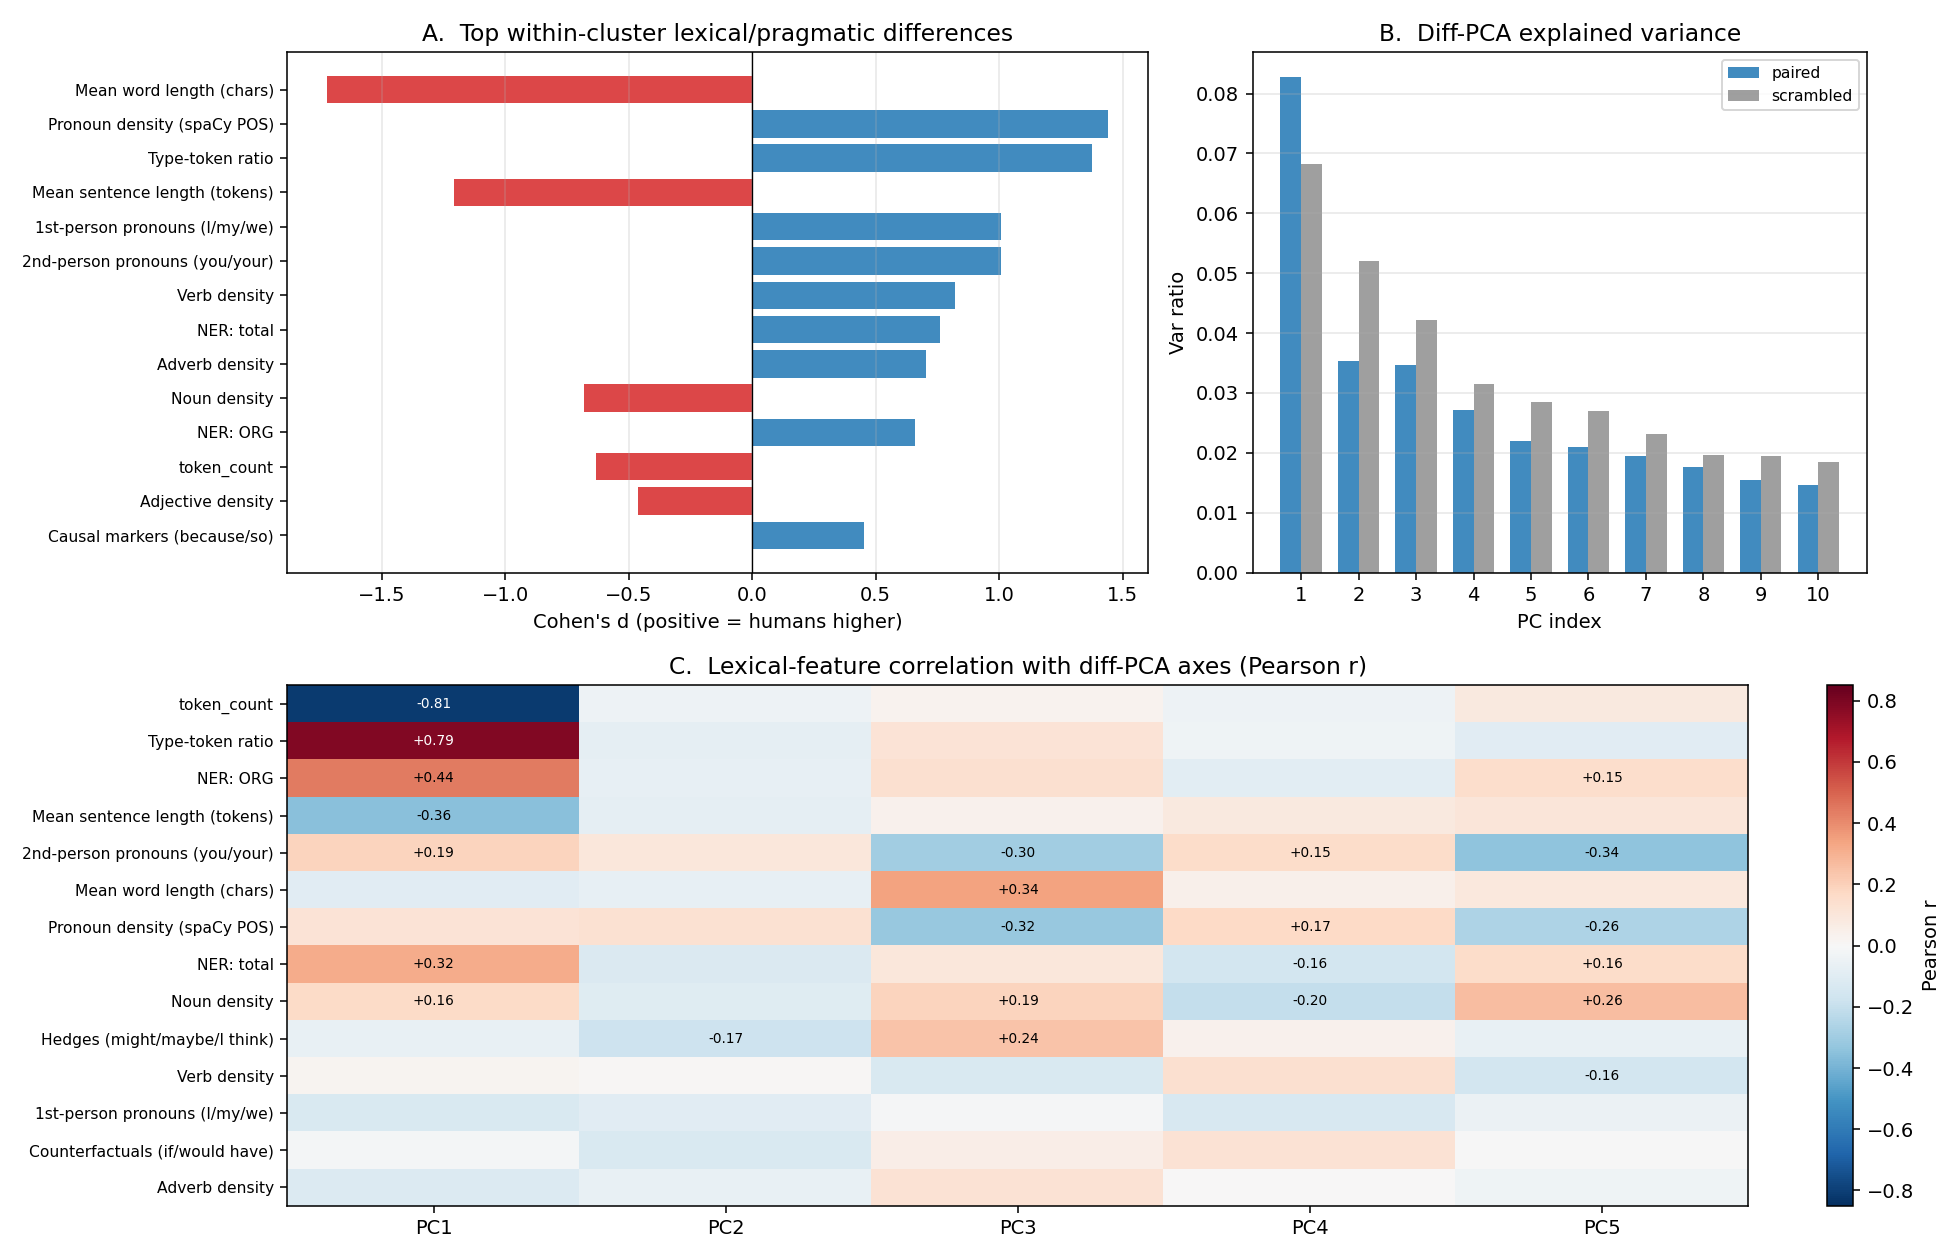
\includegraphics[width=0.92\textwidth]{milestone3_framing_figure.png}
\vspace{-0.5em}
\caption{Framing decomposition. A: top lexical and pragmatic features (Cohen's $d$, blue $=$ humans higher). B: explained variance of difference-vector PCs, paired vs random-pairing baseline. PC1 is shared (generic register), PCs 2--5 are dilemma-conditional. C: Pearson correlations between each lexical feature and each diff-vector PC.}
\label{fig:framing}
\end{figure}

%% ============================================================================
\section{Analysis}
%% ============================================================================

The corpus and per-dilemma probes give different answers. The corpus gap is multi-directional and reproduces on a 2024 model, but it is heavily register-confounded. Ridge regression on TF-IDF + length closes 91\% of it, the MFD measure reverses the Kaleido-decoder gradient, and register-matched paraphrase closes comp90 to zero. The milestone-2 ``plurality collapse'' claim oversold the corpus result.

The per-dilemma analysis recovers a content-grounded gap. Humans are $2\times$ more pairwise-diverse than LLMs in 100\% of 1,991 dilemmas and the ratio survives every surface, length, and author control. MFD foundation count is at parity, so the gap is not in which moral foundation humans invoke. At the 60-cluster Kaleido level the gap is $1.46\times$, in part because humans and LLMs choose different sub-foundation clusters. Within the same cluster the gap is still $1.95\times$, so most of the variation is in how each side elaborates a cluster both sides share. Humans are more personal, more concrete, more partisan, and more counterfactual than LLMs on the same dilemma in the same Kaleido cluster. The lexical signature is length-robust on 11 of 22 features. The PCA shows PC1 is generic register but PCs 2--5 are dilemma-conditional. The qualitative probe converges on the same axis. The within-cluster diversity is therefore neither pure moral content nor pure surface register. It is moral-expressive style below the foundation level.

%% ============================================================================
\section{Conclusions}
%% ============================================================================

\paragraph{Strengths.} The corpus gap survives matched-$n$ sampling, length quintiles, kernel PCA, a sentence-transformer encoder swap, consensus and verdict stratification, the permutation null, INLP, the per-component analysis, and generation by a 2024 model. The ArcticShift expansion adds 68,391 human comments across 1,991 dilemmas, with a $2\times$ ratio in every dilemma that survives every surface, length, and author control. The framing decomposition further shows the within-cluster residual is a coherent multidimensional style and stance axis.

\paragraph{Weaknesses.} Three independent tests show the corpus-level gap is register-dominated. Ridge regression closes 91\%, the MFD gradient reverses, and register-matched paraphrase closes comp90 to zero. None of the three is conclusive on its own (paraphrase introduces content drift, MFD is a small lexicon, TF-IDF misses some surface variation), but they converge. The corpus-level ``plurality collapse'' claim is hard to defend without a cleaner separation of register from content.

\paragraph{Limitations.} Single source (Reddit AITA), single language, single task. The seven LLMs are 2--3 generations old, but a 2024 model lives inside the old cluster. Only 62\% of rationales contain any MFD lemma, limiting the reach of that measure. The qualitative probe used a 3B judge and 38\% of its output is template.

\paragraph{Future work.} A causal log-likelihood study on OLMo-2 32B~\cite{olmo2}, which provides public base, SFT, DPO, and RLVR checkpoints. We would score the same human and LLM rationales under each checkpoint and compare $\Delta \log P$ across stages, isolating which alignment step compresses the distribution. This avoids the encoder-decoder coupling that limited milestone 2. A paired register-matched control arm and a bidirectional NLI-validated paraphrase pipeline would settle the register-vs-content question at the corpus level.

\bibliographystyle{plain}
\footnotesize
\begin{thebibliography}{9}
\bibitem{sorensen2024kaleido}
T.\ Sorensen, L.\ Jiang, J.\ Hwang, S.\ Levine, V.\ Pyatkin, P.\ West, N.\ Dziri, X.\ Lu, K.\ Rao, C.\ Bhagavatula, M.\ Sap, J.\ Tasioulas, and Y.\ Choi.
``Value Kaleidoscope: Engaging AI with Pluralistic Human Values, Rights, and Duties,'' \emph{AAAI 2024}. Model: \texttt{allenai/kaleido-xl}.
\bibitem{sachdeva2025dilemmas}
P.\ S.\ Sachdeva and T.\ van Nuenen.
``Normative Evaluation of Large Language Models with Everyday Moral Dilemmas,'' \emph{ACM FAccT 2025}. arXiv:2501.18081. Dataset: \texttt{ucberkeley-dlab/normative\_evaluation\_llms\_everyday\_dilemmas}.
\bibitem{arcticshift}
A.\ Heitmann. Arctic Shift: Reddit Historical Data Archive. \url{https://arctic-shift.photon-reddit.com}, accessed April 2026. Source: \texttt{github.com/ArthurHeitmann/arctic\_shift}.
\bibitem{qwen2025}
Qwen Team.
``Qwen2.5 Technical Report,'' arXiv:2412.15115, 2024. Model: \texttt{Qwen/Qwen2.5-3B-Instruct}.
\bibitem{reimers2019sbert}
N.\ Reimers and I.\ Gurevych.
``Sentence-BERT: Sentence Embeddings using Siamese BERT-Networks,'' \emph{EMNLP-IJCNLP 2019}, pp.\ 3982--3992. Library: \texttt{sentence-transformers}, model \texttt{all-mpnet-base-v2}.
\bibitem{graham2009moral}
J.\ Graham, J.\ Haidt, and B.\ A.\ Nosek.
``Liberals and Conservatives Rely on Different Sets of Moral Foundations,'' \emph{J.\ Personality and Social Psychology}, 96(5):1029--1046, 2009. Source of the Moral Foundations Dictionary lexicon.
\bibitem{ravfogel2020inlp}
S.\ Ravfogel, Y.\ Elazar, H.\ Gonen, M.\ Twiton, and Y.\ Goldberg.
``Null It Out: Guarding Protected Attributes by Iterative Nullspace Projection,'' \emph{ACL 2020}, pp.\ 7237--7256. arXiv:2004.07667.
\bibitem{olmo2}
OLMo Team (P.\ Walsh, L.\ Soldaini, D.\ Groeneveld et al.).
``2 OLMo 2 Furious,'' arXiv:2501.00656, 2025. Models: \texttt{allenai/OLMo-2-0325-32B-\{Base,SFT,DPO,Instruct\}}.
\end{thebibliography}

\end{document}
